% !TEX root = ../Dokumentation.tex
\section{Realisierung}
\subsection{Softwaredesing}
\subsection{Verwendete Hardware}

\begin{figure}[H]%Position festigen
\centering
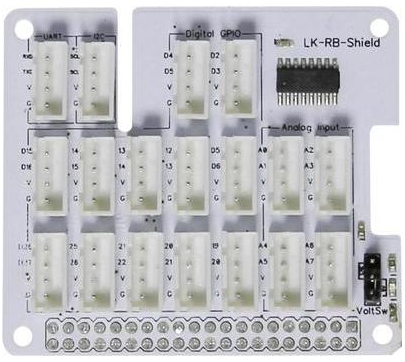
\includegraphics[width=0.25\textwidth]{Images/Basisplatine.jpg}
\caption{Basisplatine zum Raspberry Pi (Quelle www.Conrad.ch)}
\label{fig:plate}
\end{figure}

\begin{figure}[H]%Position festigen
\centering
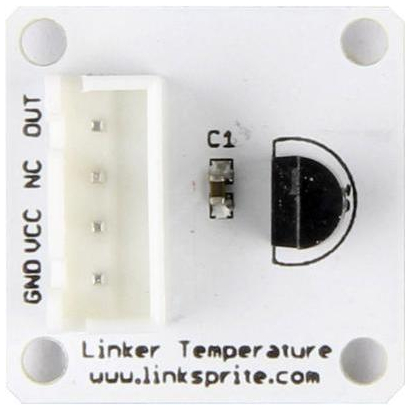
\includegraphics[width=0.25\textwidth]{Images/Sensorplatine.jpg}
\caption{Sensorplatine mit Temperaturfühler (Quelle www.Conrad.ch)}
\label{fig:sensor}
\end{figure}

\begin{figure}[H]%Position festigen
\centering
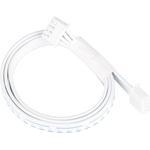
\includegraphics[width=0.25\textwidth]{Images/Verbindungskabel.jpg}
\caption{Verbindungskabel (Quelle www.Conrad.ch)}
\label{fig:cable}
\end{figure}

\subsection{Webdarstellung}

\section{Versuchsdurchführung}